\newpage
\section*{Molecular systems and cartoon conventions}
The two cases share a categorical construction, but differ in molecular
resolution and chart coordinates. Alanine dipeptide is represented by ten
heavy atoms. CLN025 is represented by ten C$\alpha$ sites, one per residue:
the equal site counts do not imply equal molecular complexity.

\begin{figure}[H]\centering
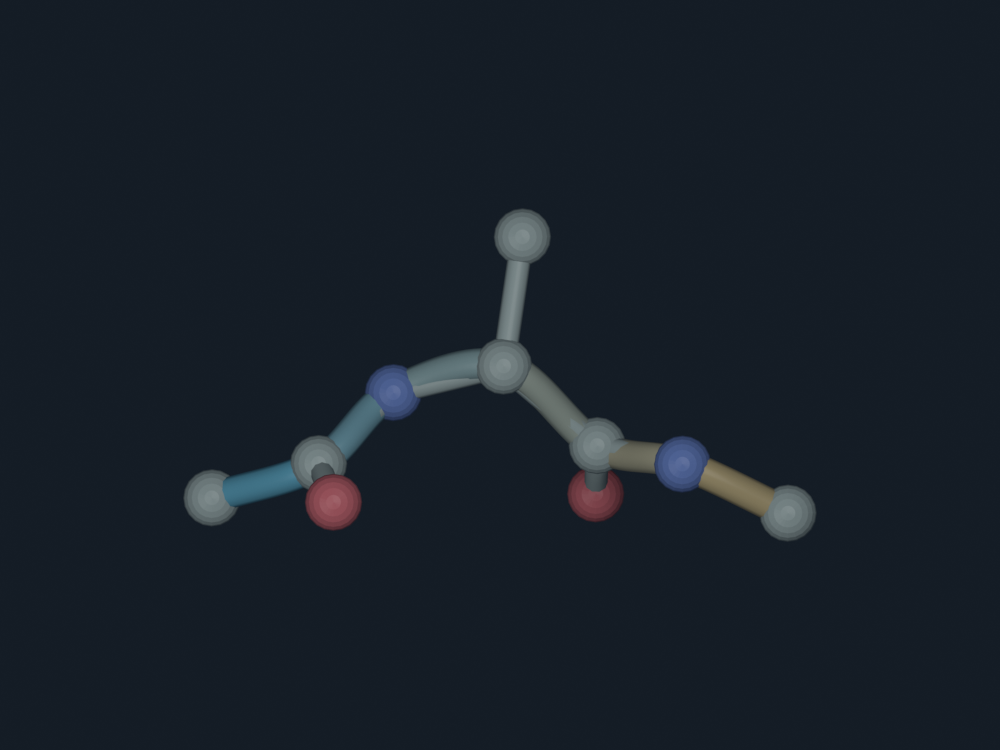
\includegraphics[width=.43\linewidth]{figures/alanine-cartoon.png}
\caption{\textbf{Alanine dipeptide: a backbone cartoon with atomic context.}
The blue-to-gold tube traces the capped backbone from one end to the other;
heavy atoms and bonds retain chemical context (oxygen red, nitrogen blue).
Coordinates come from the recorded representative of overlap object $U_0$.
A helix/sheet ribbon would not be meaningful for this short benchmark.}
\end{figure}
\begin{figure}[H]\centering
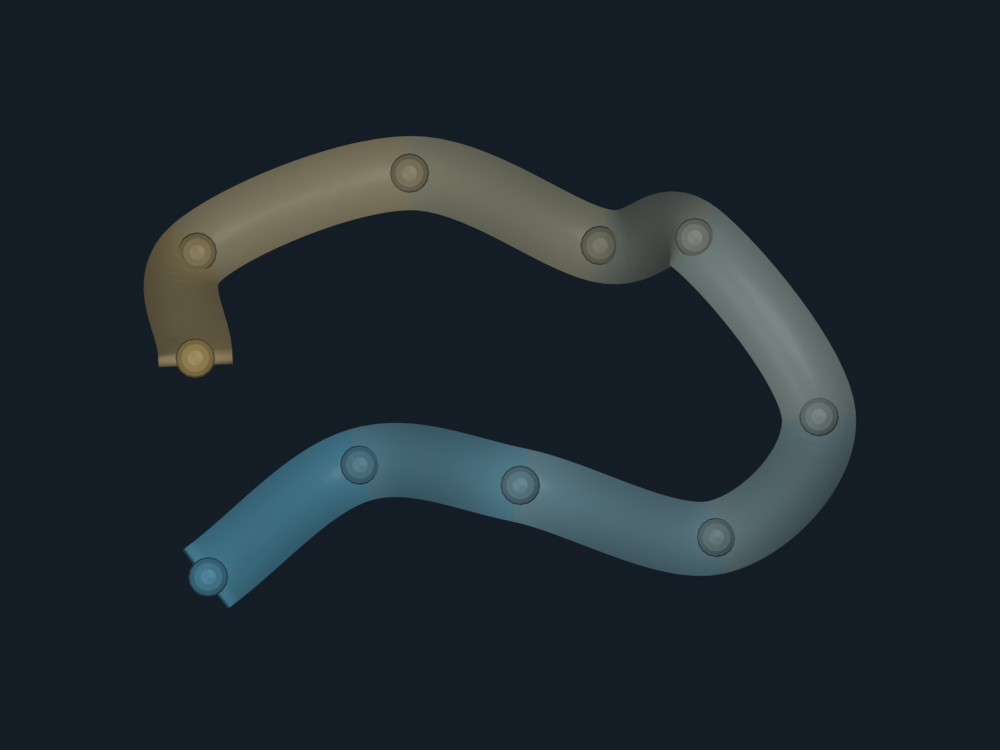
\includegraphics[width=.48\linewidth]{figures/chignolin-compact-cartoon.png}\hfill
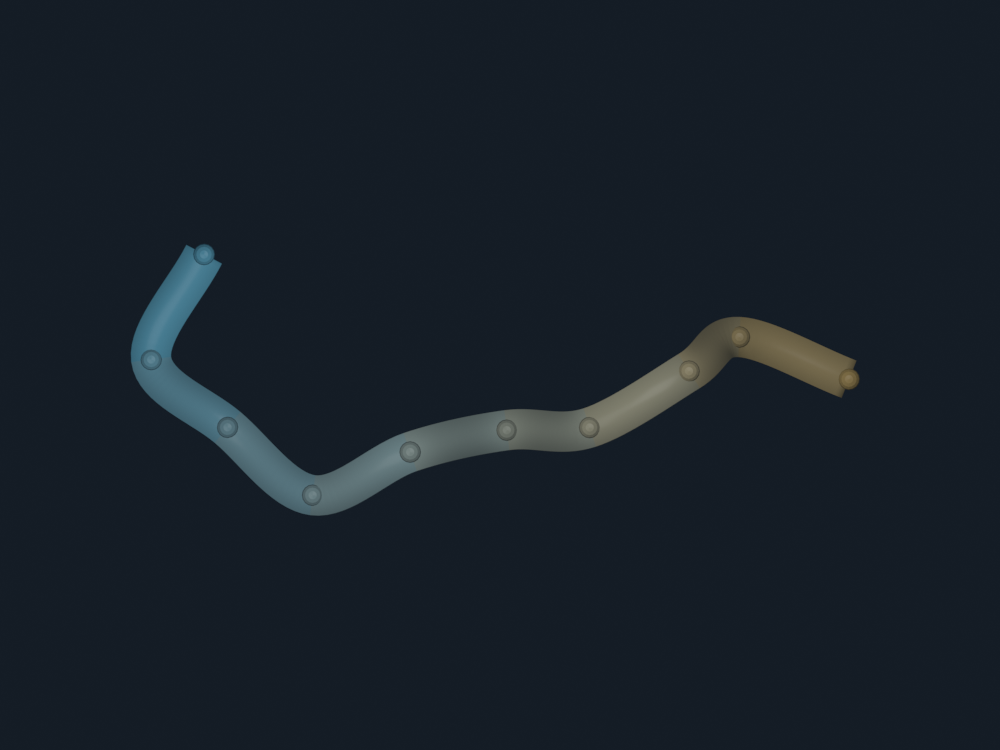
\includegraphics[width=.48\linewidth]{figures/chignolin-extended-cartoon.png}
\caption{\textbf{Chignolin CLN025: compact and extended C$\alpha$ cartoons.}
Sequence YYDPETGTWY. Actual frames nearest the 5th and 95th percentiles of
C$\alpha$ radius of gyration are shown. Ribbons interpolate the recorded
C$\alpha$ sites; blue-to-gold indicates N-to-C order. These are geometric
backbone cartoons, not DSSP secondary-structure assignments or assertions of
native and unfolded states. Each panel has its own fitted camera scale.}
\end{figure}
The cartoons and landscape figures were rendered in Blender from exported
MD coordinates. Smooth ribbons and tubes are illustrative interpolation between
sites. The CLN025 mutation and capping conventions are inherited from the
deposited simulation topology; the example is not mislabeled as wild-type
chignolin. The viewer provides corresponding backbone-trace insets, recorded
representatives, and animated route conformations.
